La mayor evidente diferencia entre el algoritmo presentado en la seccion \ref{sec:algoritmo-aternativo} y el algoritmo clásico es que en lugar de poder explorar transiciones entre estados completamente abstractos, la manera en la que explora las transiciones de la EPA implica que sólo está considerando ciertos caminos de métodos al evaluar cada transición.
Esto se debe a que en cada paso selecciona un par (método, estado abstracto) que no haya explorado ya, pero la exploración \textbf{no} considera todos los estados posibles que puedan abstraerse al estado abstracto.
En cambio, sólo puede considerarse un subconjunto de los estados que la herramienta pudo alcanzar hasta ese momento.

Consideremos el siguiente ejemplo, el contrato \texttt{BoundedStack}, cuyo código podemos ver en el fragmento de código \ref{code:solidity-bounded-stack}.
Este contrato consiste en una simple implementación de una pila como estructura de datos, con la peculiaridad de que la pila cuenta con un tamaño máximo.
El contrato tiene sólo dos métodos externos: \textcolor{orange}{\texttt{push}} y \textcolor{orange}{\texttt{pop}}.
\begin{lstlisting}[language=Solidity, label={code:solidity-bounded-stack}, caption={Contrato Inteligente \texttt{BoundedStack} en Solidity},captionpos=b]
contract SizedStack {
    uint256 public size;
    uint256 public maxSize;
    uint256[] internal_arr;
    constructor() public {
        maxSize = 10;
        size = 0;
    }
    function isEmpty() public view returns (bool) {
        return size == 0;
    }
    function top() public view returns (uint256) {
        require(!isEmpty());
        return internal_arr[size - 1];
    }
    function push(uint256 new_elem) public {
        require(size < maxSize);
        internal_arr.push(new_elem);
        size += 1;
    }
    function pop() public returns (uint256) {
        require(!isEmpty());
        uint256 was = top();
        internal_arr.pop();
        size -= 1;
        return was;
    }
}
\end{lstlisting}
La EPA de este contrato por otro lado también es bastante sencilla, y la podemos ver en la imagen \ref{fig:bounded-stack-epa}.
Por fuera de los estados \textbf{init} y \textbf{vacio}, contamos con solo tres estados alcanzables, que son \textbf{\_push}, \textbf{\_pop} y \textbf{\_push\_pop}.
El estado \textbf{\_push} se corresponde con la pila vacía, y es el que se produce al desplegar el contrato o luego de ejecutar \textcolor{orange}{\texttt{pop}} reiteradas veces.
Cuando la pila tiene elementos pero no está llena se encuentra en el estado \textbf{\_push\_pop}, al que se puede llegar tanto desde sí mismo, como desde \textbf{\_push} y desde \textbf{\_pop}.
Finalmente, el estado \textbf{\_pop} se corresponde con la pila llena, y se puede llegar tanto desde \textbf{\_push} (si el tamaño de la pila fuese uno) o desde \textbf{\_push\_pop}, pero no desde el constructor.
Notoriamente, a menos que el contrato sea deployeado con un tamaño máximo de cero, nunca será posible alcanzar el estado \textbf{\_vacio}.

Este es un buen ejemplo para observar la limitación introducida por el algoritmo alternativo al no explorar realmente todas las ejecuciones posibles de un método.
Como se representa en la figura \ref{fig:bounded-stack-bad-epa}, veremos que es posible que el análisis del contrato \texttt{BoundedStack} por el algoritmo alternativo no pueda encontrar algunas de las transiciones presentes en la EPA, dependiendo del orden en el que elija ejecutar los métodos del contrato.
Realicemos manualmente la exploración que realizaría el algoritmo para este contrato y veamos que es posible llegar al resultado presentado en la figura \ref{fig:bounded-stack-bad-epa}, en el que algunas transiciones son omitidas de la EPA.
\begin{figure}[H]
    \centering
    \begin{subfigure}{0.4\textwidth}
        {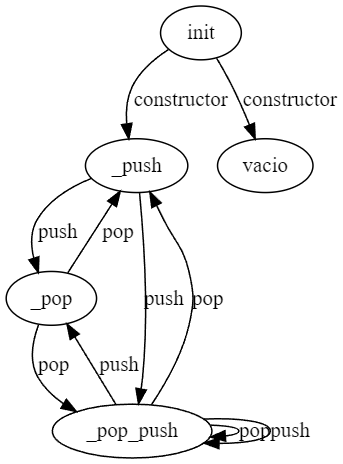
\includegraphics[width=\textwidth]{figs/bounded-stack-good-epa.png}}
        \caption{Enabledness Preserving Abstraction del contrato \texttt{BoundedStack}}
        \label{fig:bounded-stack-epa}
    \end{subfigure}
    \hfill
    \begin{subfigure}{0.4\textwidth}
        {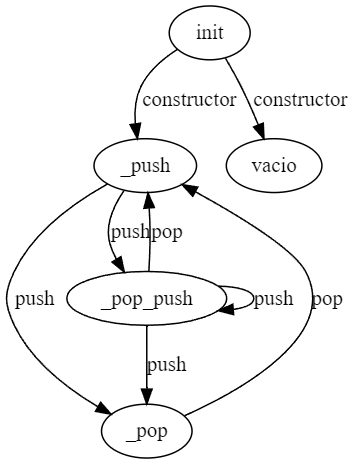
\includegraphics[width=\textwidth]{figs/bonded-stack-bad-epa.png}}
        \caption{EPA errónea del contrato \texttt{BoundedStack} generada por el algoritmo alternativo.
            No se encuentran presentes las transiciones \textbf{\_pop} a \textbf{\_push\_pop} mediante \textcolor{orange}{\texttt{pop}} ni \textbf{\_push\_pop} a \textbf{\_push\_pop} mediante \textcolor{orange}{\texttt{pop}}.}
        \label{fig:bounded-stack-bad-epa}
    \end{subfigure}
\end{figure}

El algoritmo explora los estados alcanzables comenzando desde el constructor.
Como vimos en la EPA de \texttt{BoundedStack}, los estados que resultan alcanzables son \textbf{\_push} y \textbf{vacio}.
Hasta ahora tenemos entonces $P_0 = \{\emptyset, \textbf{\_push}\}, S = \{\emptyset, \textbf{\_push}\}$ y que  $\Delta(s,m) = \emptyset$ para todos los $m$ y $s$.
Luego, el algoritmo elige un método de los disponibles a ejecutar al azar, que en este caso sería solamente \textcolor{orange}{\texttt{push}}.
Luego de ejecutar ese método, los estados que resultan alcanzables desde el estado \textbf{\_push} son \textbf{\_push\_pop} (con la restricción de que el tamaño de la pila sea mayor a uno) y \textbf{\_pop} (con la restricción de que el tamaño de la pila sea exactamente uno).
En este punto, $P_0 = \{\emptyset, \textbf{\_push}\}, S = \{\emptyset, \textbf{\_push}, \textbf{\_push\_pop}, \textbf{\_pop}\}$ y  $\Delta(\textbf{\_push},\textcolor{orange}{\texttt{push}}) = \{\textbf{\_push\_pop}, \textbf{\_pop}\}$.

Ahora, este es el punto en el que el próximo paso de la exploración del algoritmo puede cambiar el resultado final de la abstracción generada.
Por un lado, podemos elegir explorar \textcolor{orange}{\texttt{pop}} desde \textbf{\_push\_pop} y \textbf{\_pop}, marcando los pares $(\textbf{\_push\_pop},\textcolor{orange}{\texttt{pop}})$ y $(\textbf{\_pop},\textcolor{orange}{\texttt{pop}})$ como ya explorados, o explorar \textcolor{orange}{\texttt{push}} desde \textbf{\_push\_pop} y dejar la exploración de \textcolor{orange}{\texttt{push}} para más adelante.
Por otro lado se puede explorar \textcolor{orange}{\texttt{push}}, marcando el par $(\textbf{\_push\_pop},\textcolor{orange}{\texttt{push}})$.
Si continuamos la ejecución suponiendo que en este paso se elige explorar \textcolor{orange}{\texttt{pop}}, descubriremos dos transiciones nuevas: de \textbf{\_push\_pop} a \textbf{\_push} mediante \textcolor{orange}{\texttt{pop}} y de \textbf{\_pop} a \textbf{\_push} mediante \textcolor{orange}{\texttt{pop}} también.
Nos puede llamar la atención que desde los estados (concretos) que elegimos para explorar la ejecución de \textcolor{orange}{\texttt{pop}} hay dos transiciones que no podemos ver: de \textbf{\_pop} a \textbf{\_push\_pop} mediante \textcolor{orange}{\texttt{pop}} y de de \textbf{\_push\_pop} a \textbf{\_push\_pop} mediante \textcolor{orange}{\texttt{pop}}.
Estas se deben a que en este momento todos los estados concretos que estamos considerando tienen su tamaño real de la pila en 1.
Sin embargo, el algoritmo no presta atención a cuál fue la traza de métodos ejecutada para llegar hasta acá, por lo que marca a ambas tuplas $(\textbf{\_push\_pop},\textcolor{orange}{\texttt{pop}})$ y $(\textbf{\_pop},\textcolor{orange}{\texttt{pop}})$ como ya exploradas.
Esto significa que la función de transición $\Delta$ quedará definida en $\Delta(\textbf{\_push\_pop},\textcolor{orange}{\texttt{pop}}) = \textbf{\_push}$ y $\Delta(\textbf{\_pop},\textcolor{orange}{\texttt{pop}}) = \textbf{\_push}$.
De aquí en adelante la ejecución del algoritmo proseguirá hasta terminar con (al menos) esas dos transiciones faltantes.

